\subsection{Share of Detected Cases}
\label{subsec:results_share_known_cases}

We show the age group specific share of detected cases in
Figure~\ref{fig:share_known_cases_by_age_group}.\footnote{We explain how we model the
detection of cases in Section~\ref{sub:testing} and show the overall share of detected
cases that we use as input for our testing model in
Section~\ref{subsec:data_share_known_cases}.}

In 2020 the share of detected cases is much higher in older age groups as they are much
more likely to develop symptoms and symptomatic individuals are much more likely to be
tested. Starting in 2021 the share of detected cases not only depends on the overall
share of detected cases ($\psi_t$) we feed into our model but also on the number of
performed rapid tests (governed by the $\pi$ parameters). As more and more (often
asymptomatic and presymptomatic) individuals receive positive rapid tests and seek and
get confirming PCR tests, the share of detected cases starts to increase, especially
after March when rapid tests became much more widely available. This effect is very
visible for school pupils (5-14, green line). As twice weekly rapid tests become
mandatory in schools and students start going to school after the Easter break, the share
of detected cases for that group increases drastically from 25\% to over 60\% between
April and June.

\begin{figure}[ht]
  \centering
  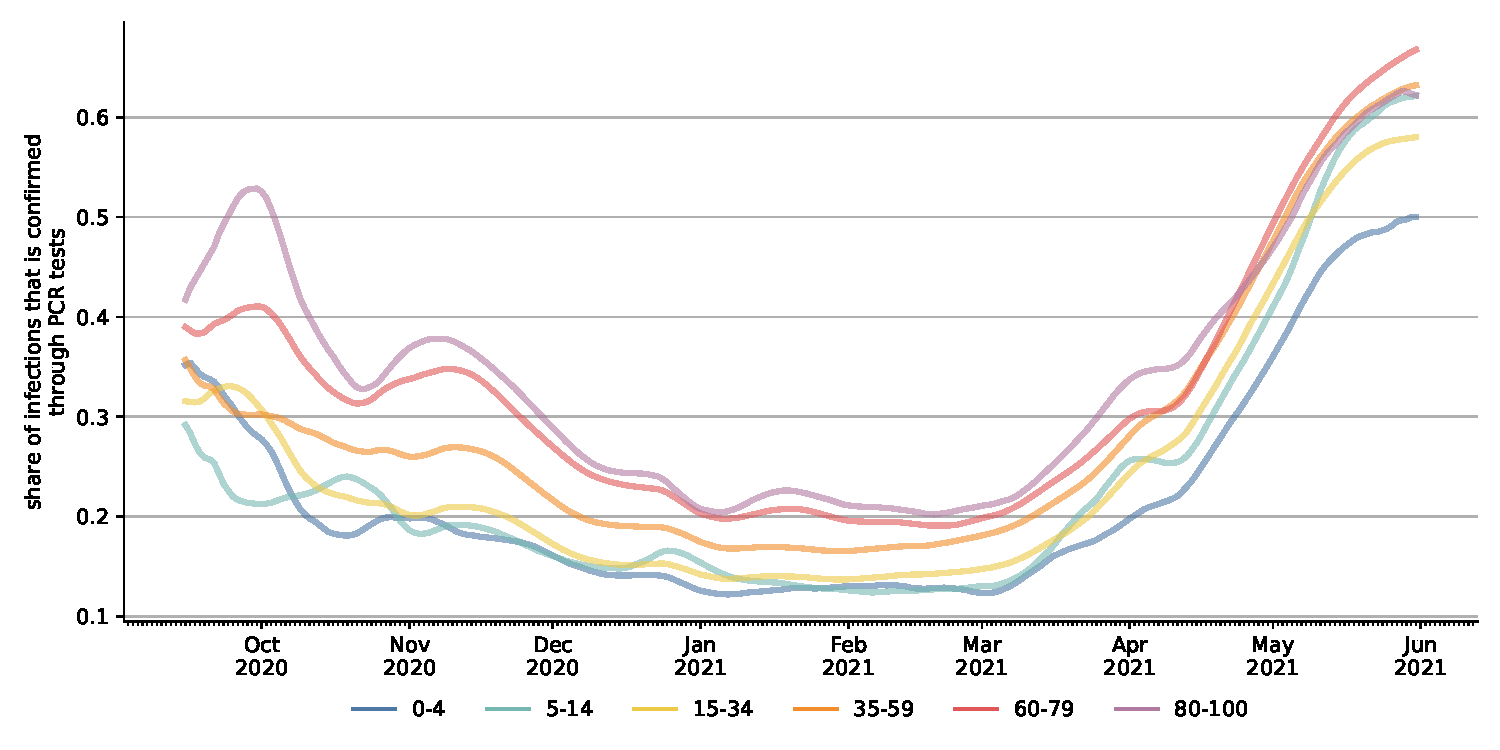
\includegraphics[width=0.5\textwidth]{figures/results/figures/share_known_cases/full_combined_baseline_by_age_group_rki}
  \caption{Share of Detected Cases by Age Group}
  \label{fig:share_known_cases_by_age_group}
  \floatfoot{\noindent \textit{Note:} The figure shows the share of cases that is
  reported as an official case via PCR confirmation for each age group in our population.
  We use the overall share of detected cases ($\psi_t$) that was estimated through the
  case fatality ratio by \citet{Dunkelzifferradar2020} for all of 2020 and then assume it
  to be constant as vaccinations of the elderly strongly affect the case fatality rate
  which the project does not account for. To get from an overall share of detected cases
  to the share of cases that is detected in each age group we use that asymptomatic cases
  are much less likely to be detected. As our model covers age specific asymptomatic
  rates this endogenously leads to group specific share of detected cases that suggest
  that infections in younger age groups are under-detected. Starting in 2021 in addition
  to the overall numbers of detected cases through $\psi_t$, cases are also detected
  through confirmation of positive rapid tests. This leads to an increase in the share of
  detected cases for all age groups but in particular for the younger age groups that are
  covered extensively with rapid tests through the rapid test requirement for
  participating in school. Age groups that have high shares of workers also have
  disproportionately increases in their detection rates.}
\end{figure}


\FloatBarrier